\section{LITERATURE REVIEWS}
\subsection{Mobile Robot Modelling}
\hspace{1.27cm}
Differential drive mobile robot is a commonly used and developed robot in the field. It is a very simple robot that operates in two wheels. Both wheels are attached to the common axis and usually are driven by two independent motors. To prevent the robot platform from tilting, one or more free spin caster wheel are attached to the robot platform. The differential drive wheel mobile robot model is illustrated in \textbf{\figureautorefname{ \ref{fig:Differential Drive Wheel Mobile Robot}}}.The differential drive robot movements depend on the velocity of each individual wheel which dictate its motion and steering. For example: if both wheels move in the same direction and at the same speed, the robot will move forward. If both wheels move in the different direction of each other but in the same speed, the robot will rotate about its center —etc.\par

% Figure Image =============================================================================
\begin{figure}[ht]
	\centering
	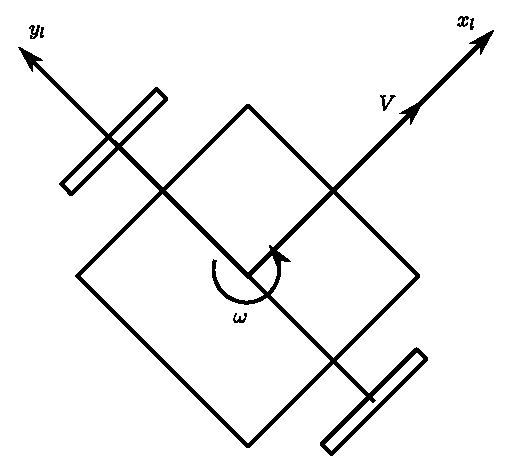
\includegraphics[scale=1]{images/imagess/2lit-DDWMR.eps} 
	\caption{Differential Drive Wheel Mobile Robot}
	\label{fig:Differential Drive Wheel Mobile Robot}
\end{figure}
% Figure Image =============================================================================

\hspace{1.27cm}
Differential drive mobile robot pose is represented in the 2D Cartesian coordinate system. There are two coordinate frames that the robot uses, the global frame and the local frame. In kinematic, the robot velocity is described using two variables and vice versa it is used to control input to the robot. The variables are:\par

\begin{itemize}
\item \(V\), the linear velocity along the x-axis of the local coordinate frame
\item \(\omega\), the angular velocity about the z-axis of the local coordinate frame.
\end{itemize}






\break
\subsection{Controller}
\hspace{1.27cm}
The differential drive mobile robot is a nonholonomic constraint system due to the absence of the velocity along the Y-axis of the local frame. 
The nonholonomic constraint of the robot is:
\begin{equation}
-\Dot{x} sin\theta + \Dot{y} cos\theta = 0
\end{equation}

\textbf{\figureautorefname{ \ref{fig:Mobile Robot Navigation}}} shows a common navigation of mobile robot. To achieve the control of the nonholonomic constraint system, the use of a nonsmooth or time varying controller is needed because the system is nonlinear and varies in time. The robot system is divided into kinematic control and dynamics control. The Most commonly used controls for mobile robots are:
\begin{itemize}
\item \textbf{Control to reference pose}\\
is the control approach where the reference position and orientation is predefined. From the current pose to the reference pose, the robot can drive in an arbitrary path.
\item \textbf{Control to segment of line}\\
is the control approach where the reference segment of the line is constructed from multiple reference poses.
\item \textbf{Control to reference trajectory}\\
is the control approach where the reference pose is a function of time. 
\end{itemize}
\par 

% Figure Image =============================================================================
\begin{figure}[ht]
	\centering
	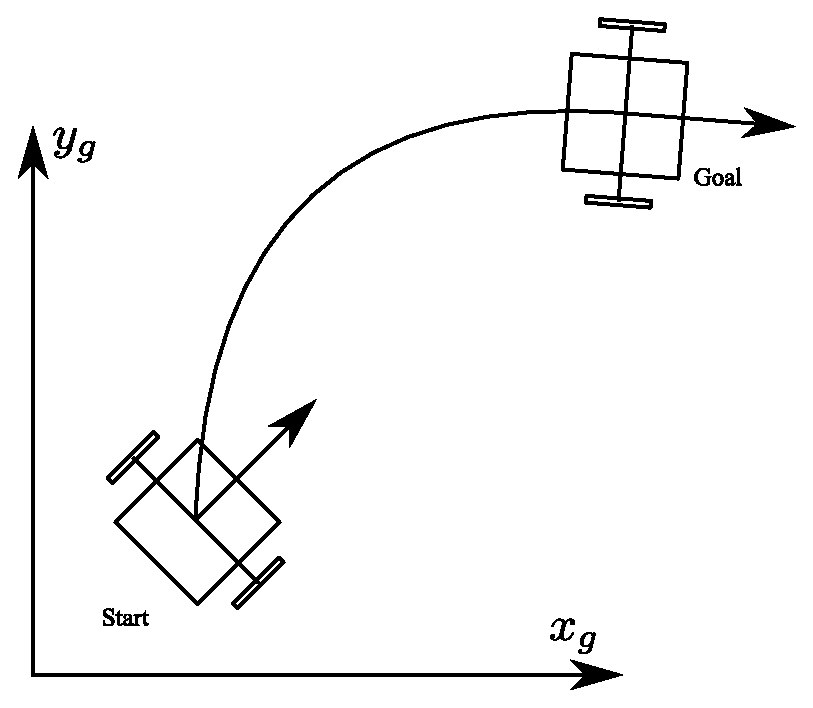
\includegraphics[scale=0.8]{images/imagess/2lit-MRNav.eps} 
	\caption{Mobile Robot Navigation}
	\label{fig:Mobile Robot Navigation}
\end{figure}
% Figure Image =============================================================================

\hspace{1.27cm}
Control wheel mobile robots usually decompose into two part: the \textbf{Feedforward} control and the \textbf{Feedback} control as illustrated in \textbf{\figureautorefname{ \ref{fig:Simple Feedforward and Feedback control}}}.
\begin{itemize}
    \item In \textbf{Feedforward} control, the input to control robot is determined from the calculation of the reference goal or trajectory. The input can then apply to the robot system to move along in the open-loop system.
    \item On the other hand, the \textbf{Feedback} control determine the current state of the robot in every time step and feeds back to the controller for a robust performance.
\end{itemize}
\par

% Figure Image =============================================================================
\begin{figure}[ht]
	\centering
	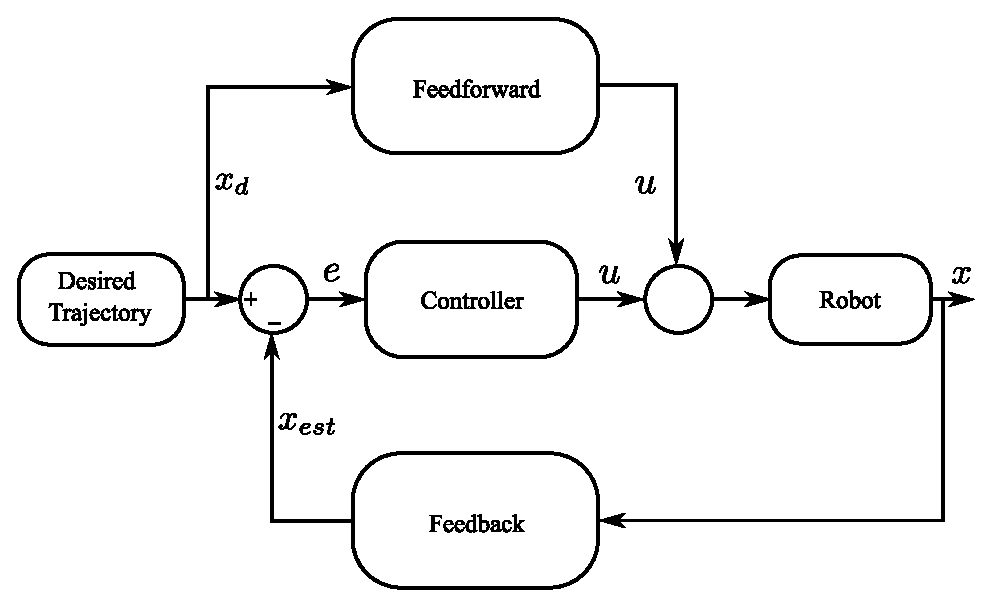
\includegraphics[scale=1]{images/imagess/2lit-simplecontrl.eps} 
	\caption{Simple Feedforward and Feedback control}
	\label{fig:Simple Feedforward and Feedback control}
\end{figure}
% Figure Image =============================================================================

\hspace{1.27cm}
In the real world, the mobile robot is a dynamics system. Thus, for robust control on the dynamics system, the dynamic properties of the system are included, such as torque, mass, moment of inertia, external force acting on the robot,-etc.\\
The controller of the robot dynamics system can be decomposed into two parts: the \textbf{Outer} controller and the \textbf{Inner} controller.
\begin{itemize}
    \item For the \textbf{outer} controller, the system calculate the required system velocities to move along the reference trajectory or to move to a reference pose. 
    \item While the \textbf{inner} control is calculating the torque or force that is required to match the required system velocity from the outer controller.
\end{itemize}
\par














\subsection{Path Planning}

% Figure Image =============================================================================
\begin{figure}[ht]
	\centering
	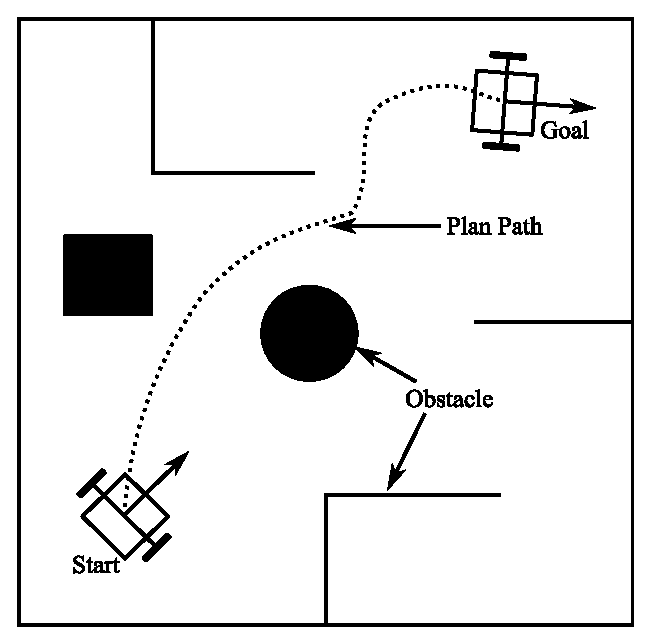
\includegraphics[scale=1]{images/imagess/2lit-pathplan.eps} 
	\caption{Path Planning}
	\label{fig:Path Planning}
\end{figure}
% Figure Image =============================================================================

\hspace{1.27cm}
To reach a certain goal, the robot required a number of information and algorithms to perform. In the process of path planning, the robot computes sequence of valid actions of the robot configuration to move to the goal. In the case of a mobile robot, the problem is usually defined as the moving from start to goal while avoiding the obstacle \textbf{\figureautorefname{ \ref{fig:Path Planning}}}. In the process of path planning of the real world scenario, the robot’s kinematic and dynamic constraints is considered. Since the environment is not always the same, the path planning works with the limited of the representation of the environment in the algorithm. The algorithm can perform in a fully or partly known environment.\par

\hspace{1.27cm}
A preliminary literature review show that there are many approaches to the problem. For example:

$\bullet$ \textbf{Probabilistic Road Maps (PRMs)}

\begin{itemize}
    \item \textbf{Random Space Sampling}\\
    the algorithm indicates the random points in space that are selected to construct a graph, whose edges are created if two nodes abstain no more than a certain distance.\\
    \item \textbf{Space Sampling with Halton Sequence}\\
    a graph is created by selecting points in space using Halton sequence.
    \item \textbf{Uniform Space Sampling}\\
    the algorithm selects even points in the free space at a certain step. Each selected node is connected to eight peripheral sampling points.
\end{itemize}

$\bullet$ \textbf{Visibility Graph}\par
Visibility graph construction is based on the environment's convex obstacles as the algorithm treats their edges as possible nodes. A Ray Casting technique is utilized in order for the robot to perceive the obstacles' edges. As ray detection method has not been expanded as much as the others, the ending point is stored as an obstacle edge, which is the node in the graph. When one node can connect to the other without the graph's edge intersecting an obstacle, the nodes' connections in graph is established.

$\bullet$ \textbf{Rapidly exploring Random Trees — RRTs}
\begin{itemize}
    \item \textbf{Standard RRT}\\
    a random point in the free space is selected. Then, the current constructed tree is checked in order for its closest node to the random point in free space to be found.
    \item \textbf{Star RRT}\\
    the algorithm aim to improve the method of Standard RRT due to highly random path.
    \item \textbf{Multiple RRTs}\\
    the algorithm aim to speed the convergence of Standard RRT
\end{itemize}

$\bullet$ \textbf{Generalized Voronoi Diagram}\par
Generalized Voronoi Diagram is constructed by a set of points in the free space which abstain evenly from the environment's obstacle if the Manhattan distance is taken into account as metric. \par

$\bullet$ \textbf{A* Planning}\par
the algorithm determines the path based on the path cost and cost estimation required to extend the path until the goal using the cost function.\par

Each of the algorithms has their own advantages and disadvantages considered on the computation time and robustness.(\cite{duchovn2014path}) (\cite{inproceedings})
\par

%\break
%\hspace{1.27cm}
%The path planning algorithm introduce the concept of configuration and configuration space. Configuration represents the state of the system in the environment space in n dimension. The state vector is described by $q = [q_1,...,q_n]^T$.The state q is a point in n-dimensional space called configuration space Q, which presents all possible configurations of the mobile system according to its kinematic model. Part of the configuration space that is occupied by the obstacles $O_i$ is denoted $Q_{obst} = \cup_i O_i $. Thus, the part of the environment is \[Q_{free} = Q - Q_{obst}\]